\documentclass{article}
\usepackage[utf8]{inputenc} %кодировка
\usepackage[T2A]{fontenc}
\usepackage[english,russian]{babel} %русификатор 
\usepackage{mathtools} %библиотека матеши
\usepackage[left=1cm,right=1cm,top=2cm,bottom=2cm,bindingoffset=0cm]{geometry} %изменение отступов на листе
\usepackage{amsmath}
\usepackage{graphicx} %библиотека для графики и картинок
\graphicspath{}
\DeclareGraphicsExtensions{.pdf,.png,.jpg}
\usepackage{subcaption}
\usepackage{pgfplots}
\usepackage{float}
\usepackage{amssymb}
\usepackage{physics}

\begin{document}
% НАЧАЛО ТИТУЛЬНОГО ЛИСТА
\begin{center}
    \Large
    Федеральное государственное автономное \\
    образовательное учреждение высшего образования \\ 
    «Научно-образовательная корпорация ИТМО»\\
    \vspace{0.5cm}
    \large
    Факультет программной инженерии и компьютерной техники \\
    Направление подготовки 09.03.04 Программная инженерия \\
    \vspace{1cm}
    \Large
    \textbf{Отчёт по лабораторной работе №5} \\
    По дисциплине «Методы оптимизации» (4 семестр)\\
    \large
    \vspace{8cm}

    \begin{minipage}{.33\textwidth}
    \end{minipage}
    \hfill
    \begin{minipage}{.4\textwidth}
    
        \textbf{Студент}: \vspace{.1cm} \\
        \ Дениченко Александр P3212\\
        \textbf{Практик}:  \\
        \ Селина Елена Георгиевна
    \end{minipage}
    \vfill
Санкт-Петербург\\ 2024 г.
\end{center}
\pagestyle{empty}
% КОНЕЦ ТИТУЛЬНОГО ЛИСТА 
\newpage
\pagestyle{plain}


\section*{Задание 1}
Данные\\
\[\begin{cases}
    -2x_1 - 3x_2 -> min,\\
    2x_1-3x_2\geq 12,\\
    x_1+x_2\geq2,\\
    3x_1+6x_2 \leq 24,\\
    x_1,x_2\geq 0
\end{cases}\]
Решить задачу линейного программирования графическим методом. 
\\ \\
Изобразим на плоскости допустимое множество X данной задачи (треугольник) и одну из линий уровня целевой
функции (чёрный цвет, где функция задана: $-2x_1 - 3x_2 = -14$).

\begin{center}
    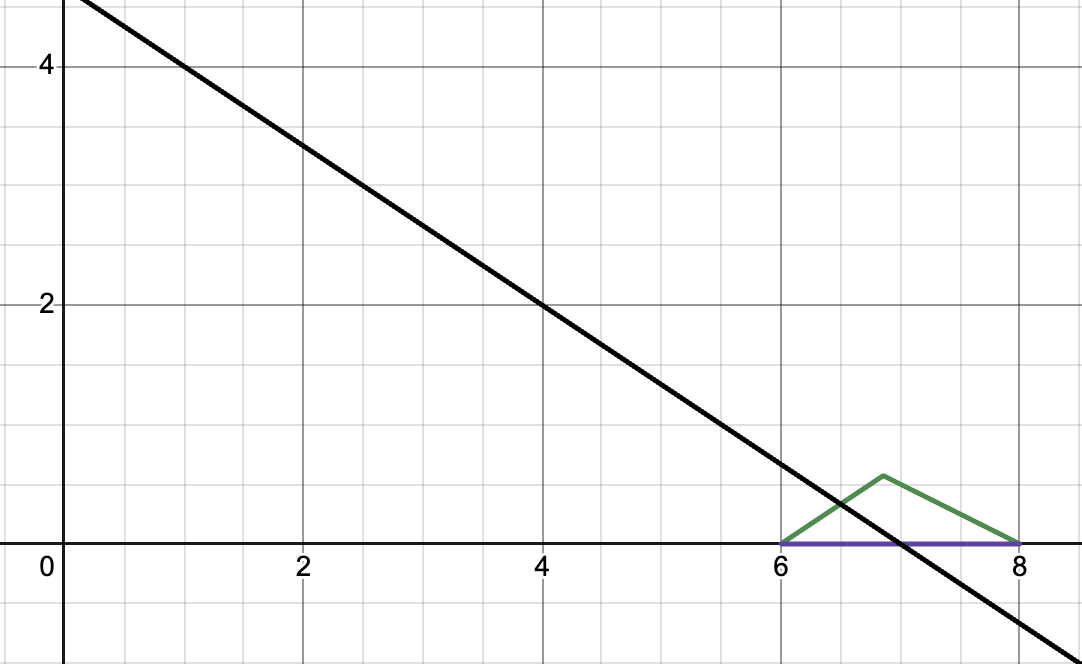
\includegraphics[width=.7\textwidth]{func.png}
\end{center}
Антиградиент
\[-\grad f(x) = (2, 3) = \overline{e}\]
\begin{center}
    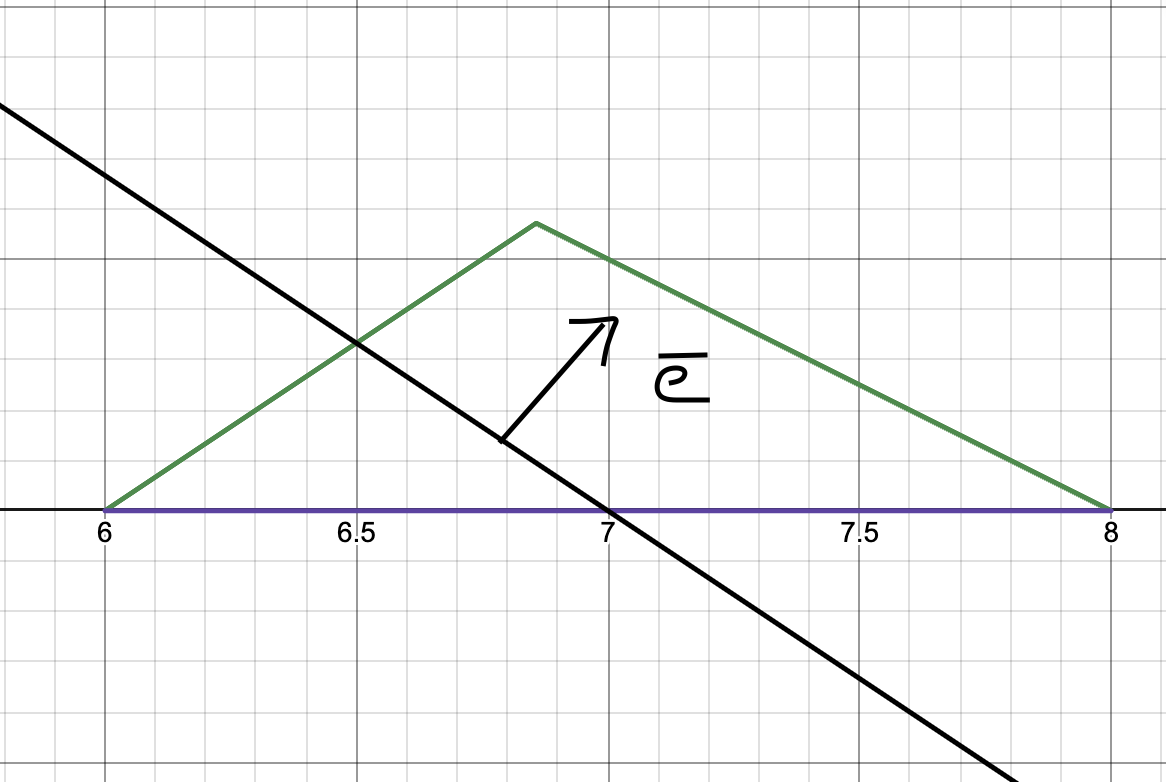
\includegraphics[width=.5\textwidth]{grad.png}
\end{center}
указывает направление убывания функции. 
Совершая параллельный перенос линии уровня вдоль напрвления находим её крайнее положение.
\begin{center}
    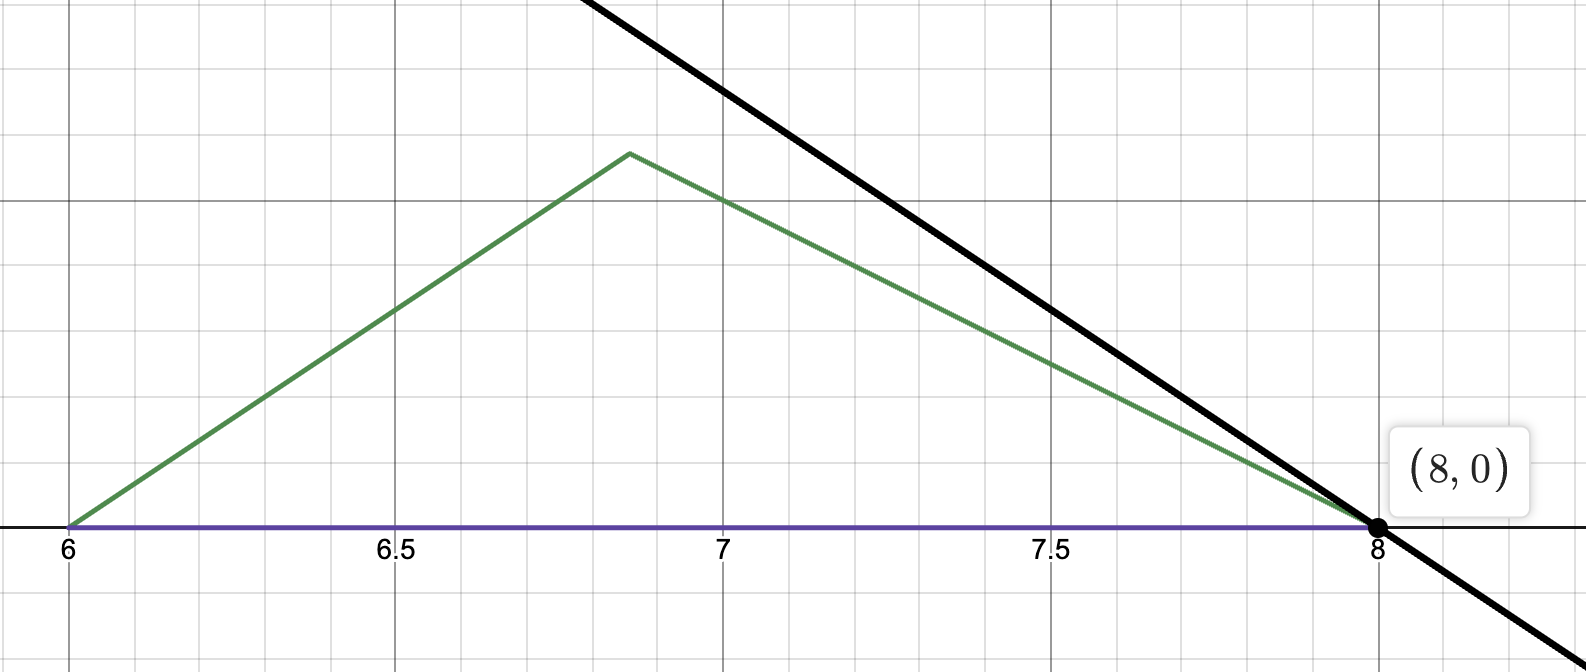
\includegraphics[width=.5\textwidth]{min.png}
\end{center}
В этом положении прямая проходит через вершину с координатами (8, 0).
Поэтому целевая функция f(x) принимает единственное значение в точке x = (8, 0).
\[f^* = -2\cdot 8 - 3\cdot 0 = -16\]

\section*{Задание 2}
Даны матрица А и векторы c и b. Решить каноническую задачу линейного программирования
\[f(x) = cx \ -> max\]
при ограничениях
\[Ax = b,\ x\geq 0\]
с помощью симплекс-метода.
\\ \\
\[c = (0, 1, -6, 1, -3),\ b = (9, 14, 3)\]
\[A = \begin{pmatrix}
    6&1&1&2&1\\
    -1&0&-1&7&8\\
    1&0&2&1&1
\end{pmatrix}\]
Перепишем в удобный вид
\[f(x) = x_2-6x_3+x_4-3x_5\]
\[\begin{cases}
    6x_1+x_2+x_3+2x_4+x_5 = 9\\
    -x_1-x_3+7x_4+8x_5 = 14\\
    x_1+2x_3+x_4+x_5 = 3\\
    x_i \geq 0,\ x_i = 1, ..., 5
\end{cases}\]
Ищем начальное базисное решение:
Столбец 2 является частью единичной матрицы. Переменная пусть x2 входит в начальный базис.
\begin{table}[H]
    \centering
    \caption{Начальная симплекс-таблица}
    \begin{tabular}{|c|c|c|c|c|c|c|}
    \hline
        базис & $x_1$ & $x_2$ & $x_3$ & $x_4$ & $x_5$ & b \\ \hline
        $x_2$ & 6 & 1 & 1 & 2 & 1 & 9 \\
        ? & -1 & 0 & -3 & 7 & 8 & 14 \\
        ? & 1 & 0 & 2 & 1 & 1 & 3 \\ \hline
    \end{tabular}
\end{table}
В качестве ещё одной базисной переменной берём x1. 

\begin{table}[H]
    \centering
    \caption{Добавление в базис x1}
    \begin{tabular}{|c|c|c|c|c|c|c|}
    \hline
        базис & $x_1$ & $x_2$ & $x_3$ & $x_4$ & $x_5$ & b \\ \hline
        $x_2$ & 6&	1	&1	&2	&1&	9 \\
        $x_1$ & -1&	0&	-3&	7	&8&	14 \\
        ? & 1	&0	&2	&1&	1&	3 \\ \hline
    \end{tabular}
\end{table}
Преобразование: Делим строку 2 на -1. Из строк 1, 3 вычитаем строку 2, умноженную на соответствующий элемент в столбце 1.

\begin{table}[H]
    \centering
    \caption{Преобразование для x1}
    \begin{tabular}{|c|c|c|c|c|c|c|}
    \hline
        базис & $x_1$ & $x_2$ & $x_3$ & $x_4$ & $x_5$ & b \\ \hline
        $x_2$ & 0	&1&	-17	&44&	49&	93 \\
        $x_1$ & 1&	0&	3	&-7	&-8	&-14 \\
        $x_3$  & 0	&0	&-1&	8	&9	&17 \\ \hline
    \end{tabular}
\end{table}

В качестве ещё одной базисной переменной берём x3.
\begin{table}[H]
    \centering
    \caption{Добавление в базис x3}
    \begin{tabular}{|c|c|c|c|c|c|c|}
    \hline
        базис & $x_1$ & $x_2$ & $x_3$ & $x_4$ & $x_5$ & b \\ \hline
        $x_2$ & 0	&1&	-17	&44&	49&	93 \\
        $x_1$ & 1&	0&	3	&-7	&-8	&-14 \\
        $x_3$  & 0	&0	&-1&	8	&9	&17 \\ \hline
    \end{tabular}
\end{table}

Преобразование: Делим строку 3 на -1. Из строк 1, 2 вычитаем строку 3, умноженную на соответствующий элемент в столбце 3.

\begin{table}[H]
    \centering
    \caption{Преобразование для x3}
    \begin{tabular}{|c|c|c|c|c|c|c|}
    \hline
        базис & $x_1$ & $x_2$ & $x_3$ & $x_4$ & $x_5$ & b \\ \hline
        $x_2$ & 0	&1&	0	&-92&	-104	&-196 \\
        $x_1$ & 1	&0&	0	&17	&19&	37 \\
        $x_3$  & 0&0	&1	&-8	&-9	&-17 \\ \hline
    \end{tabular}
\end{table}

В столбце b присутствуют отрицательные значения. Максимальное по модулю $|b|_{max}$ = 196 находится в строке 1. 
Максимальный по модулю элемент в 1 строке -104 находится в столбце 5. 
Тогда в качестве базисной переменной x2 берём x5.

Преобразование: Делим строку 1 на -104. Из строк 2, 3 вычитаем строку 1, умноженную на соответствующий элемент в столбце 5.

\begin{table}[H]
    \centering
    \caption{Преобразование для x5}
    \begin{tabular}{|c|c|c|c|c|c|c|}
    \hline
        базис & $x_1$ & $x_2$ & $x_3$ & $x_4$ & $x_5$ & b \\ \hline
        $x_5$ & 0	&-$\frac{1}{104}$&	0	&$\frac{23}{26}$&	1	&$\frac{49}{26}$ \\
          &	&&	&&		&\\\hline
        $x_1$ & 1	&$\frac{19}{104}$&	0	&$\frac{5}{26}$	&0&	$\frac{31}{26}$ \\
        &	&&	&&		&\\\hline
        $x_3$  & 0&-$\frac{9}{104}$	&1	&-$\frac{1}{26}$&0	&-$\frac{1}{26}$ \\ 
        &	&&	&&		&\\\hline
    \end{tabular}
\end{table}
В столбце b присутствуют отрицательные значения.
Максимальное по модулю $|b|_{max}$ = |$-\frac{1}{26}$| находится в строке 3.
Максимальный по модулю элемент в 3 строке $-\frac{9}{104}$ находится в столбце 2.
Выберем в качестве базисной переменной x3 - x2.

Преобразование: Делим строку 3 на $-\frac{9}{104}$. 
Из строк 1, 2 вычитаем строку 3, умноженную на соответствующий элемент в столбце 2.
\begin{table}[H]
    \centering
    \caption{Преобразование для x2}
    \begin{tabular}{|c|c|c|c|c|c|c|}
    \hline
        базис & $x_1$ & $x_2$ & $x_3$ & $x_4$ & $x_5$ & b \\ \hline
        $x_5$ & 0	&0&	-$\frac{1}{9}$	&$\frac{8}{9}$&	1	&$\frac{17}{9}$ \\
          &	&&	&&		&\\\hline
        $x_1$ & 1	&0&	$\frac{19}{9}$	&$\frac{1}{9}$	&0&	$\frac{10}{9}$ \\
        &	&&	&&		&\\\hline
        $x_2$  & 0&1	&-$\frac{104}{9}$	&$\frac{4}{9}$&0	&$\frac{4}{9}$ \\ 
        &	&&	&&		&\\\hline
    \end{tabular}
\end{table}

Восстановим функцию:
\[f(x) = x_2-6x_3+x_4-3x_5\]

\[f(x) = (\frac{104}{9}x_3 - \frac{4}{9}x_4 + \frac{4}{9})-6x_3+x_4-3\cdot (\frac{1}{9}x_3 - \frac{8}{9}x_4 + \frac{17}{9}) = \frac{47}{9}x_3+\frac{29}{9}x_4-\frac{47}{9}\]

Симплекс таблица:

\begin{table}[H]
    \centering
    \caption{Расчёт строки f}
    \begin{tabular}{|c|c|c|c|c|c|c|}
    \hline
        базис & $x_1$ & $x_2$ & $x_3$ & $x_4$ & $x_5$ & b \\ \hline
        $x_5$ & 0	&0&	-$\frac{1}{9}$	&$\frac{8}{9}$&	1	&$\frac{17}{9}$ \\
          &	&&	&&		&\\\hline
        $x_1$ & 1	&0&	$\frac{19}{9}$	&$\frac{1}{9}$	&0&	$\frac{10}{9}$ \\
        &	&&	&&		&\\\hline
        $x_2$  & 0&1	&-$\frac{104}{9}$	&$\frac{4}{9}$&0	&$\frac{4}{9}$ \\ 
        &	&&	&&		&\\\hline
        $f$  & -&-	&$\frac{47}{9}$	&$ \frac{29}{9}$&-	&$-\frac{47}{9}$ \\ 
        &	&&	&&		&\\\hline
    \end{tabular}
\end{table}
\[\Delta_1 > 0, \Delta_2 > 0\ \ => \ \ \text{критерий оптимальности не выполнен} \]
Продолжим поиск. Берём максимально положительный столбец с $f = \frac{47}{9}$. 

\[min\left(-\frac{\frac{17}{9}}{-\frac{1}{9}}, -\frac{\frac{10}{9}}{\frac{19}{9}}, -\frac{\frac{4}{9}}{-\frac{104}{9}}\right) = (17, -\frac{10}{19}, \frac{1}{26}) = -\frac{10}{19} \]


\[x_1 = \frac{19}{9}x_3 + \frac{1}{9}x_4 + \frac{10}{9}\]

В базис идёт x3 вместо x1.
\[x_3 = \frac{9}{19}x_1 -\frac{1}{19}x_4 - \frac{10}{19}\]
\[x_5 = -\frac{1}{9}\cdot(\frac{9}{19}x_1 -\frac{1}{19}x_4 - \frac{10}{19}) + \frac{8}{9}x_4 + \frac{17}{9} = 
-\frac{1}{19}x_1 + \frac{17}{19}x_4 + \frac{37}{19}\]
\[x_2 = -\frac{104}{9}\cdot(\frac{9}{19}x_1 -\frac{1}{19}x_4 - \frac{10}{19}) + \frac{4}{9}x_4+ \frac{4}{9} = 
-\frac{109}{19}x_1 + \frac{20}{19}x_4 + \frac{124}{19}\]

Подсчитаем функцию:

\[f(x) = (-\frac{109}{19}x_1 + \frac{20}{19}x_4 + \frac{124}{19})-6\cdot(\frac{9}{19}x_1 -\frac{1}{19}x_4 - \frac{10}{19})+x_4-3\cdot (-\frac{1}{19}x_1 + \frac{17}{19}x_4 + \frac{37}{19}) =\]
\[= -\frac{160}{19}x_1 - \frac{6}{19}x_4 + \frac{73}{19}\]
\begin{table}[H]
    \centering
    \caption{Замена x1 на x3}
    \begin{tabular}{|c|c|c|c|c|c|c|}
    \hline
        базис & $x_1$ & $x_2$ & $x_3$ & $x_4$ & $x_5$ & b \\ \hline
        $x_5$ & $-\frac{1}{19}$	&0&	0	&$\frac{17}{19}$&	1	&$\frac{37}{19}$ \\
          &	&&	&&		&\\\hline
        $x_3$ & $\frac{9}{19}$	&0&	1	&$-\frac{1}{19}$	&0&	$- \frac{10}{19}$ \\
        &	&&	&&		&\\\hline
        $x_2$  & $-\frac{109}{19}$&1	&0	&$\frac{20}{19}$&0	&$\frac{124}{19}$ \\ 
        &	&&	&&		&\\\hline
        $f$  & $-\frac{160}{19}$&-	&-	&$ - \frac{6}{19}$&-	&$\frac{73}{19}$ \\ 
        &	&&	&&		&\\\hline
    \end{tabular}
\end{table}
Критерий оптимальности выполнен.
Ответ:
\[x_2 = \frac{124}{19}\]
\[x_3 = -\frac{10}{19}\]
\[x_5 = \frac{37}{19}\]
\[f_{max} = \frac{73}{19}\]

\section*{Задание 3}

Данные:
\[C = (-\frac{1}{3}, -\frac{1}{2}, 0, 0, 0)\]
\[b = (-3, -1 ,-5)\]
\[A = \begin{pmatrix}
    -4&2&0&0&2\\
    2&-4&2&0&0\\
    -2&-2&0&2&0
\end{pmatrix}\]
Прямая задача:
\[max(CX|AX = b^T,\ x\geq 0)\]

\[\begin{cases}
    -4x_1+2x_2+2x_5 = -3\\
    2x_1 -4x_2+2x_3 = -1\\
    -2x_1-2x_2+2x_4 = -5
\end{cases}\]

\[f(x) = -\frac{1}{3}x_1 - \frac{1}{2}x_2\ ->\ max\]
Построим двойственную задачу: 
\[min(b\lambda | A^T \lambda \geq c^T,\ \lambda \geq 0)\]
\[A^T = \begin{pmatrix}
    -4&2&-2\\
    2&-4&-2\\
    0&2&0\\
    0&0&2\\
    2&0&0
\end{pmatrix}\]
Двойственная задача имеет вид:
\[g(\lambda) = -3\lambda_1 - \lambda_2 - 5\lambda_3\ ->\ min\]

\[\begin{cases}
    -4\lambda_1 + 2\lambda_2 -2\lambda_3 \geq -\frac{1}{3}\\
    2\lambda_1 -4\lambda_2 -2\lambda_3 \geq -\frac{1}{2}\\
    2\lambda_2 \geq 0\\
    2\lambda_3 \geq 0\\
    2\lambda_1 \geq 0\\
\end{cases}\ ->\ 
\begin{cases}
    -4\lambda_1 + 2\lambda_2 -2\lambda_3 \geq -\frac{1}{3}\\
    2\lambda_1 -4\lambda_2 -2\lambda_3 \geq -\frac{1}{2}\\
    \lambda_{1, ..., 3} \geq 0\\
\end{cases}
\]
\[min(-3\lambda_1 - \lambda_2 - 5\lambda_3) = - max(3\lambda_1 + \lambda_2 + 5\lambda_3)\]
Приведём к каноническому виду, введя дополнительные перменные $\lambda_4,\ \lambda_5$:
\[
\begin{cases}
    -4\lambda_1 + 2\lambda_2 -2\lambda_3 - \lambda_4 = -\frac{1}{3}\\
    2\lambda_1 -4\lambda_2 -2\lambda_3 - \lambda_5 = -\frac{1}{2}\\
    \lambda_{1, ..., 3} \geq 0\\
\end{cases}
\ ->\ 
\begin{cases}
    4\lambda_1 - 2\lambda_2 + 2\lambda_3 + \lambda_4 = \frac{1}{3}\\
    - 2\lambda_1 + 4\lambda_2 + 2\lambda_3 + \lambda_5 = \frac{1}{2}\\
    \lambda_{1, ..., 3} \geq 0\\
\end{cases}
\]
\[\lambda_4 = -4\lambda_1 + 2\lambda_2 - 2\lambda_3 + \frac{1}{3}\]
\[ \lambda_5 =  2\lambda_1 - 4\lambda_2 - 2\lambda_3 +\frac{1}{2}\]
\[g'(\lambda) = 3\lambda_1 + \lambda_2 + 5\lambda_3\]

\begin{table}[H]
    \centering
    \caption{Построение начальной симплекс таблицы}
    \begin{tabular}{|c|c|c|c|c|}
    \hline
    &$\lambda_1$&$\lambda_2$&$\lambda_3$&$\beta$\\\hline
    $\lambda_4$&-4&2&-2&$\frac{1}{3}$\\
    &&&&\\\hline
    $\lambda_5$&2&-4&-2&$\frac{1}{2}$\\
    &&&&\\\hline
    $g'$&3&1&5&0\\
    &&&&\\\hline
    \end{tabular}
\end{table}
Критерий оптимальности не выполнен 
\[min(\frac{1}{6}, \frac{1}{4}) = \frac{1}{4}\]
 $\lambda_3$ попадает в базисные, а $\lambda_5$ попадает в свободные перменные.
\[\lambda_5 = 2\lambda_1 -4\lambda_2-2\lambda_3 +\frac{1}{2}\]

\[\lambda_3 = \lambda_1 - 2 \lambda_2 - \frac{1}{2}\lambda_5 +\frac{1}{4} \]
\[\lambda_4 = -4\lambda_1 +2\lambda_2-2\cdot (\lambda_1 - 2 \lambda_2 - \frac{1}{2}\lambda_5 +\frac{1}{4}) + \frac{1}{2} = -6\lambda_1 +6\lambda_2+\lambda_5\]
\[g'(\lambda) = 3\lambda_1 + \lambda_2 + 5\cdot(\lambda_1 - 2 \lambda_2 - \frac{1}{2}\lambda_5 +\frac{1}{4}) =8\lambda_1 - 9\lambda_2-\frac{5}{2}\lambda_5+\frac{5}{4}\]

\begin{table}[H]
    \centering
    \caption{Симплекс таблица после смены базиса с $\lambda_3$}
    \begin{tabular}{|c|c|c|c|c|}
    \hline
    &$\lambda_1$&$\lambda_2$&$\lambda_5$&$\beta$\\\hline
    $\lambda_4$&-6&6&1&0\\
    &&&&\\\hline
    $\lambda_3$&1&-2&$-\frac{1}{2}$&$\frac{1}{4}$\\
    &&&&\\\hline
    $g'$&8&-9&$-\frac{5}{2}$&$\frac{5}{4}$\\
    &&&&\\\hline
    \end{tabular}
\end{table}
Критерий оптимальности не выполнен 
\[min(0, -\frac{1}{4}) = -\frac{1}{4}\]
$\lambda_1$ попадает в базисные, а $\lambda_3$ попадает в свободные перменные.

\[\lambda_3 = \lambda_1 - 2 \lambda_2 - \frac{1}{2}\lambda_5 +\frac{1}{4} \]

\[\lambda_1 = 2\lambda_2 + \lambda_3 +\frac{1}{2}\lambda_5 -\frac{1}{4}\]
\[\lambda_4 = -6\cdot(2\lambda_2 + \lambda_3 +\frac{1}{2}\lambda_5 -\frac{1}{4}) +6\lambda_2+\lambda_5 = -6\lambda_2-6\lambda_3-2\lambda_5 +\frac{3}{2}\]

\[g'(\lambda) = 3\cdot (2\lambda_2 + \lambda_3 +\frac{1}{2}\lambda_5 -\frac{1}{4}) + \lambda_2 + 5\lambda_3 = 7\lambda_2 +8\lambda_3 +\frac{3}{2}\lambda_5 - \frac{3}{4}\]

\begin{table}[H]
    \centering
    \caption{Симплекс таблица после смены базиса с $\lambda_1$}
    \begin{tabular}{|c|c|c|c|c|}
    \hline
    &$\lambda_2$&$\lambda_3$&$\lambda_5$&$\beta$\\\hline
    $\lambda_4$&-6&-6&-2&$\frac{3}{2}$\\
    &&&&\\\hline
    $\lambda_1$&2&1&$\frac{1}{2}$&$-\frac{1}{4}$\\
    &&&&\\\hline
    $g'$&7&8&$\frac{3}{2}$&$-\frac{3}{4}$\\
    &&&&\\\hline
    \end{tabular}
\end{table}
Критерий оптимальности не выполнен 
\[min(\frac{1}{4}, \frac{1}{4}) = \frac{1}{4}\]
$\lambda_2$ попадает в базисные, а $\lambda_4$ попадает в свободные перменные.

\[\lambda_4 = -6\lambda_2-6\lambda_3-2\lambda_5 +\frac{3}{2}\]

\[\lambda_2 = -\lambda_3 - \frac{1}{6}\lambda_4 - \frac{1}{3}\lambda_5 +\frac{1}{4}\]
\[\lambda_1 = 2(-\lambda_3 - \frac{1}{6}\lambda_4 - \frac{1}{3}\lambda_5 +\frac{1}{4})+ \lambda_3 +\frac{1}{2}\lambda_5 -\frac{1}{4} =
-\lambda_3 - \frac{1}{3}\lambda_4 - \frac{1}{6}\lambda_5 + \frac{1}{4}\]

\[g'(\lambda) = 7\cdot(-\lambda_3 - \frac{1}{6}\lambda_4 - \frac{1}{3}\lambda_5 +\frac{1}{4}) +8\lambda_3 +\frac{3}{2}\lambda_5 - \frac{3}{4} = \lambda_3 - \frac{7}{6}\lambda_4 - \frac{5}{6}\lambda_5 +1 \]

\begin{table}[H]
    \centering
    \caption{Симплекс таблица после смены базиса с $\lambda_2$}
    \begin{tabular}{|c|c|c|c|c|}
    \hline
    &$\lambda_3$&$\lambda_4$&$\lambda_5$&$\beta$\\\hline
    $\lambda_2$&-1&$-\frac{1}{6}$&$-\frac{1}{3}$&$\frac{1}{4}$\\
    &&&&\\\hline
    $\lambda_1$&-1&$-\frac{1}{3}$&$-\frac{1}{6}$&$\frac{1}{4}$\\
    &&&&\\\hline
    $g'$&1&$-\frac{7}{6}$&$-\frac{5}{6}$&$1$\\
    &&&&\\\hline
    \end{tabular}
\end{table}

Критерий оптимальности не выполнен 
\[min(\frac{1}{4}, -\frac{1}{4}) = -\frac{1}{4}\]
$\lambda_3$ попадает в базисные, а $\lambda_1$ попадает в свободные перменные.
\[\lambda_1 = -\lambda_3 - \frac{1}{3}\lambda_4 - \frac{1}{6}\lambda_5 + \frac{1}{4}\]

\[\lambda_3 = -\lambda_1-\frac{1}{3}\lambda_4-\frac{1}{6}\lambda_5+\frac{1}{4}\]
\[\lambda_2 = -(-\lambda_1-\frac{1}{3}\lambda_4-\frac{1}{6}\lambda_5+\frac{1}{4}) - \frac{1}{6}\lambda_4 - \frac{1}{3}\lambda_5 +\frac{1}{4} =
\lambda_1 + \frac{1}{6}\lambda_4-\frac{1}{6}\lambda_5\]
\[g'(\lambda) = (-\lambda_1-\frac{1}{3}\lambda_4-\frac{1}{6}\lambda_5+\frac{1}{4}) - \frac{7}{6}\lambda_4 - \frac{5}{6}\lambda_5 +1 = 
-\lambda_1 - \frac{3}{2}\lambda_4 - \lambda_5+\frac{5}{4}\]

\begin{table}[H]
    \centering
    \caption{Симплекс таблица после смены базиса с $\lambda_3$}
    \begin{tabular}{|c|c|c|c|c|}
    \hline
    &$\lambda_1$&$\lambda_4$&$\lambda_5$&$\beta$\\\hline
    $\lambda_2$&1&$\frac{1}{6}$&$-\frac{1}{6}$&$0$\\
    &&&&\\\hline
    $\lambda_3$&-1&$-\frac{1}{3}$&$-\frac{1}{6}$&$\frac{1}{4}$\\
    &&&&\\\hline
    $g'$&-1&$-\frac{3}{2}$&-1&$\frac{5}{4}$\\
    &&&&\\\hline
    \end{tabular}
\end{table}
Критерий выполнен.

Ответ:
\[\lambda_2 = 0;\ \ \lambda_3 = \frac{1}{4}; \ \ g(\lambda) = \frac{5}{4}\]


\end{document}
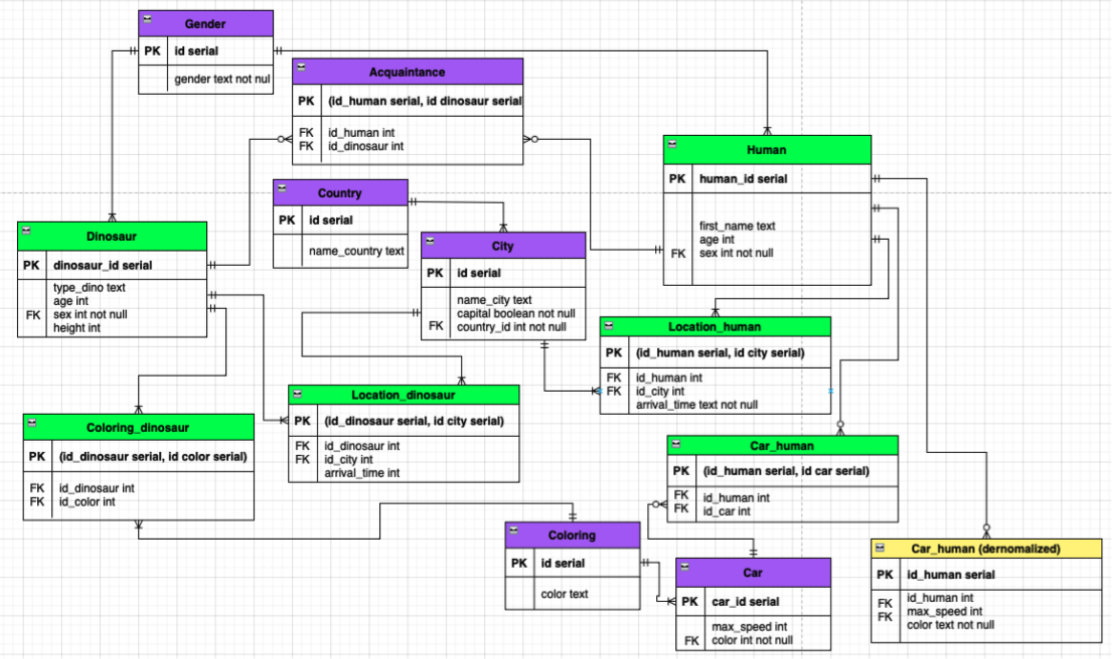
\includegraphics[width=.9\textwidth]{123}